\usetikzlibrary{automata,positioning}
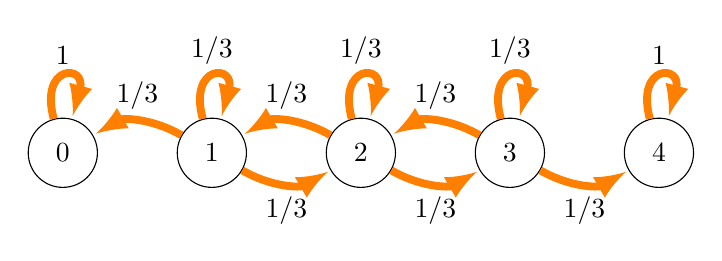
\begin{tikzpicture}

    % Add the states
    \node[state]             (s0) {0};
    \node[state, right=of s0] (s1) {1};
    \node[state, right=of s1] (s2) {2};
    \node[state, right=of s2] (s3) {3};
    \node[state, right=of s3] (s4) {4};
    % Connect the states with arrows
    \draw[every loop,auto=right,line width=1mm,>=latex,draw=orange, fill=orange]
      	(s0) edge[loop above]             node {1} (s0)
        (s1) edge[bend right, auto=right] node {1/3} (s0)
        (s1) edge[loop above]             node {1/3} (s1)
        (s1) edge[bend right, auto=right] node {1/3} (s2)
        (s2) edge[bend right, auto=right] node {1/3} (s1)
        (s2) edge[loop above]             node {1/3} (s2)
        (s2) edge[bend right, auto=right] node {1/3} (s3)
        (s3) edge[bend right, auto=right] node {1/3} (s2)
        (s3) edge[loop above]             node {1/3} (s3)
        (s3) edge[bend right, auto=right] node {1/3} (s4)
        (s4) edge[loop above]             node {1} (s4);
        
\end{tikzpicture}
